\chapter{Early experiments}

\epigraph{And you may ask yourself \\ "Well\dots how did I get here?"}{Once in a Lifetime \\ Talking Heads, 1981}

In this chapter I showcase early experiments in the different fields I worked on this thesis, with a strong focus on the different aspects of my education and artistic practice.  I include many of my breakthroughs and pitfalls that eventually led me to working on this thesis, in an open, detailed, celebratory, and critical narrative.

\section{Learning microcontrollers}

I learned how to program microcontrollers around 2010 in Chile as an undergraduate student of electrical engineering. I was taught how to program PIC microcontrollers with Microsoft's tools, including the operating system Windows and the C\# programming language. Around the same time, with my classmate Braulio we made our first project with an Arduino Uno microcontroller. It consisted of a robotic guitar tuner, where the Arduino detected the pitch of a string, analyzed the frequency, and then made a servo motor move the tuning gear of the string, in order to match the desired pitch.

\begin{figure}[ht]
  \centering
  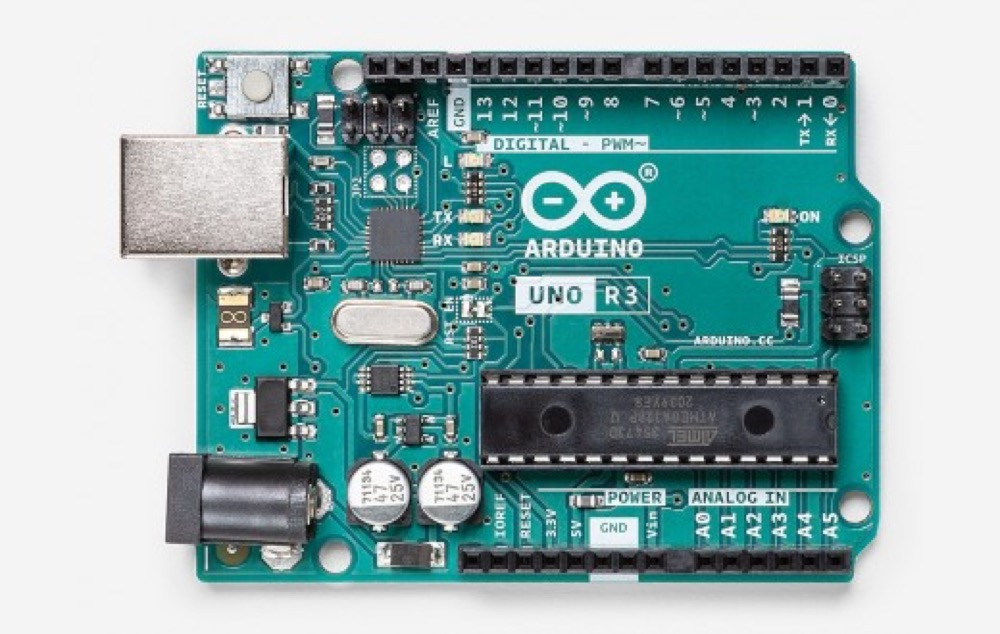
\includegraphics[width=0.75\linewidth,height=0.25\textheight,keepaspectratio]{images/arduino-uno.jpg}
  \caption{Arduino Uno microcontroller}
  \caption*{Retrieved from \cite{website-arduino-uno}}
  \label{fig:arduino-uno}
\end{figure}

Fast forward to 2013, for my undergraduate thesis I had to complete a capstone project and implement many low-level programming techniques, and Arduinos were not allowed because they were considered a shortcut. For this thesis I worked with my classmate Guillermo, and we built a robotic device with a \acrshort{PIC} microcontroller programmed with C\#. Our code was very specific to that particular chip and project, and hardly reusable or interesting for a wider audience.

Since graduation I haven't programmed with \acrshort{PIC} microcontrollers. I realized I wasn't excited about making one-off devices, with non-reusable code that I couldn't share, or having to use propietary or bulky interfaces for writing for deploying my code. In contrast, Arduinos became a huge part of my practice, because of their low cost, open source nature, ease of programming and uploadin the code with a generic USB cable, and because of the enormouus and growing available documentation and user contributed libraries, which now also includie the TinyTrainable library developed for this thesis project.

The Arduino ecosystem fostered many aspects of my practice, and now looking at it in retrospective, it made me realize that what I Love is not computers but computation, making small machines that can crunch numbers for art, and making them openly and in collaboration with friends.

A huge argument that I see people on the internet making against Arduino microcontrollers, is that they are too expensive ( ~30.00 USD) in comparison to the 1/10th of the cost of the bare bones chips and parts you need to build your own microcontroller unit. I am against this argument, since it invisibilizes the effort put in documentation by the Arduino community, and also it assumes that everybody is comfortable soldering and with high advanced electronics degrees. Even if you factor in the cost of hours you need to make your own, it doesn't pay itself. Obviously I see and the educational aspect of building your own things, but it's a slippery slope and discrimination to think that if you build a project with an Arduino it's not good because it's not from scratch, and I think it's rude t say it's not worth it, as rude as yelling at someone buying bread and making fun of them not buying the ingredients and cooking it themselves.

Another strong argument againt Arduino microcontrollers is about efficiency: that Arduino is too high-level and overbloated, and that applications and projects could be faster if you programmed on a lower-level language. I also see this argument when comparing different programming languages for graphic arts. Once again, knowing how to program with lower-level programming languages is amazing, and there is value and fun on it, but in my practice, I put a high value on my time and energy, and I rather make my code slower or less efficient, so I can spend more time making art or resting.

I rather we all have non painful programming experiences, so that we can spend more time away from screens and making art!

\section{Computer music and physical computing}

During undergrad I took classes and did research with professors and computer musicians Rodrigo Cádiz and Patricio de la Cuadra. With them I learned the fundamentals of computer music, including languages such as Max and Pure Data, which I still use to this day. For a class project I created a spoon synthesizer with masking tape, cardboard, and a Makey Makey, a device created in 2021 by Eric Rosenbaum and Jay Silver from MIT Media Lab's Lifelong Kindergarten research group. This was my first hands-on introduction to physical computing, as a way of building my own custom playful interfaces for manipulating sound with computers.
 
\begin{figure}[ht]
  \centering
  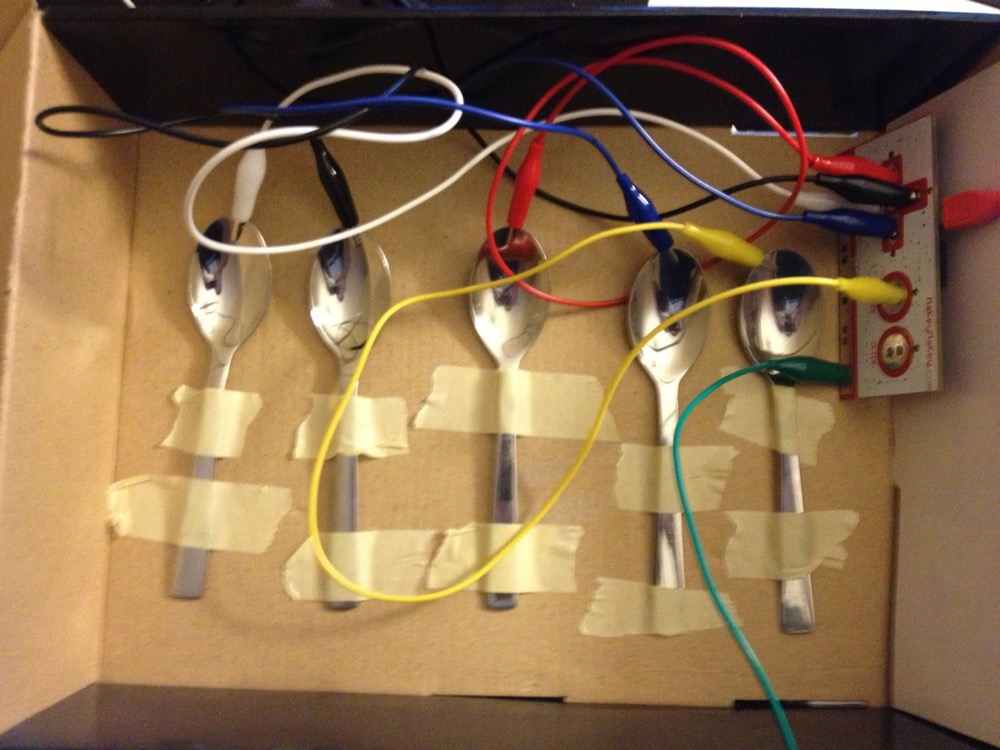
\includegraphics[width=0.75\linewidth,height=0.25\textheight,keepaspectratio]{images/makey-makey-spoons.jpg}
  \caption{Spoons and Makey Makey synthesizer}
  \caption*{Picture taken by myself}
  \label{fig:makey-makey-spoons}
\end{figure}

For this project I applied my practice as a guitar player, where I am constantly mixing and matching different devices on my pedalboard. This inspired me to make this flexible synthesizer with objects lying around me: spoons, masking tape, and cardboard. They also are forgiving, and I was able to change their physical position. The Makey Makey acted as interface with the computer, where I could assign on the fly different sounds to each spae.

In retrospective this project was an instrument an amazing experience that followed Mitchel Resnick's 4 P's: it was a Passion Project that I built for Playing with my Peers, whic is a constant on my artistic practice.

\section{Physical computing and more microcontrollers}

After graduation in 2013 I freelanced as a software and technology designer and developer for artists. I learned computer protocols and networks, and wrote custom software for live multimedia theater and music shows. Realizing that I wanted a bigger community of people to learn media arts with, I applied to New York University's Interactive Telecommunications Program (\acrshort{NYU} \acrshort{ITP}), where I joined as a graduate student in 2015. In my first semester I took the class Introduction to Physical Computing, taught by one of Arduino's co-creators Tom Igoe. Since I was already familiar with electronics and circuits, I focused on learning interface design, human computer interaction, open source hardware and software, and physical computing education.

During my research I was introduced to a wider ecosystem of microcontrollers beyond Arduino, that were possible because of its open source nature and the community behind it. My favorite example is the Teensy by PJRC, which captivated me by two main features: it can send and receive \acrshort{MIDI} over USB, and it has a powerful audio library, that allows you to play audio samples, create effects, and process real time audio. With the Teensy I was able to make standalone projects in a way that before would have required me to use a full fledged computer.

\begin{figure}[ht]
  \centering
  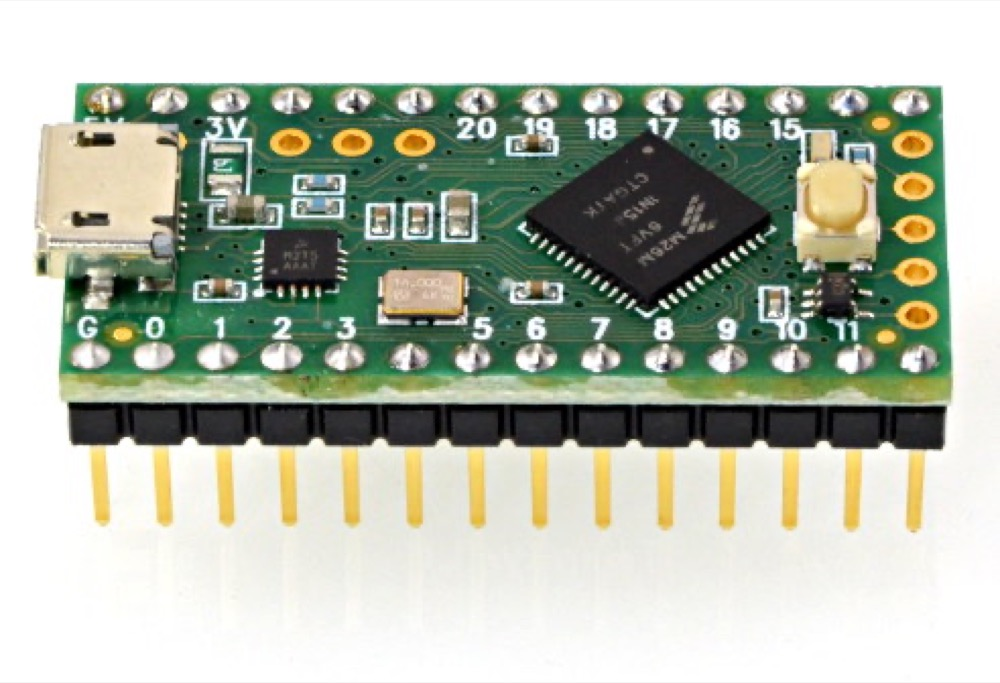
\includegraphics[width=0.75\linewidth,height=0.25\textheight,keepaspectratio]{images/pjrc-teensy-lc-with-pins.jpg}
  \caption{PJRC Teensy LC microcontroller with pins}
  \caption*{Retrieved from \cite{website-pjrc-teensy-lc-with-pins}}
  \label{fig:pjrc-teensy-lc-with-pins}
\end{figure}

\section{Processing, p5.js, Processing Foundation}

Processing is an open source software written in Java, and it was started at MIT Media Lab's Aesthetics and Computations group by Ben Fry and Casey Reas. Over the years I have learned on my own Processing, and through it computer graphics and interactivity.

I was excited to learn more Processing in 2015 in my first semester at \acrshort{NYU} \acrshort{ITP}'s Introduction to Computational Media class, like it had been taught for around a decade. I consider myself lucky, because that year they replaced the curriculum in Processing with a new one based on p5.js, another software library supported by the Processing Foundation.

p5.js was created by Lauren McCarthy as an reinterpration of Processing, using JavaScript instead of Java, to make art that runs on web browsers and over the internet. With p5.js I learned artistic and creative ways to program web applications, and this experience led me to focus on educational outreach with the Processing Foundation, which I will mention on the next section.

I was not only in awe of p5.js and Processing, but also of the people and the communities behind these software libraries. I took Lauren McCarthy's Performing User class \cite{website-nyu-itp-lauren-mccarthy-performing-user} at \acrshort{NYU} \acrshort{ITP}, and it was my favorite class during my master's. She fostered a safe space for us to explore societal and political implications of software, and it led me to add more of my personal convictions, and my body, to my artwork. This class inspired me to make a self portrait, with a countdown timer to my projected death time according to the United Nations' estimates. The first version I did was a Processing app running on a Raspberry Pi computer, and I also ported it to p5.js for web access.

\begin{figure}[ht]
  \centering
  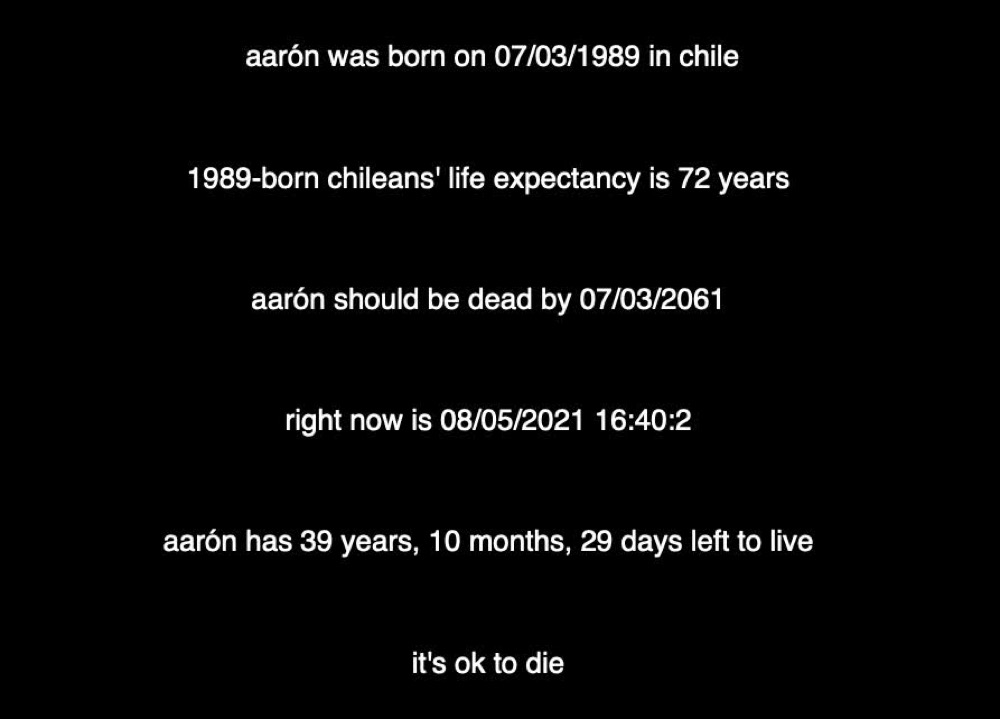
\includegraphics[width=0.75\linewidth,height=0.35\textheight,keepaspectratio]{images/its-ok-to-die-p5js.jpg}
  \caption{PJRC Teensy LC microcontroller with pins}
  \caption*{its-ok-to-die, on a browser with p5.js}
  \label{fig:its-ok-to-die-p5js}
\end{figure}

\begin{figure}[ht]
  \centering
  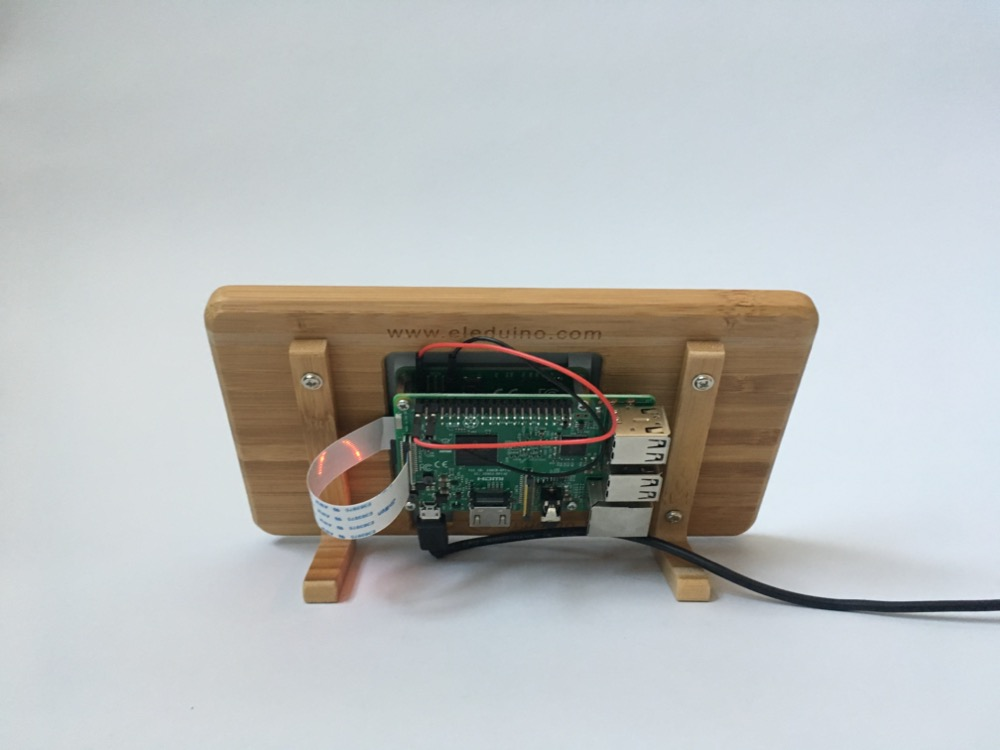
\includegraphics[width=0.75\linewidth,height=0.35\textheight,keepaspectratio]{images/its-ok-to-die-raspberry.jpg}
  \caption{its-ok-to-die, on a Raspberry Pi computer}
  \caption*{Picture taken by myself}
  \label{fig:its-ok-to-die-raspberry}
\end{figure}

\section{Teaching media arts}

While I was a student at \acrshort{NYU} \acrshort{ITP} I was the recipient of 2 summer grants to work on an internationalization project of p5.js. Since my native language is Spanish, and I wanted to share all my passion for web programming with p5.js, I focused on translating the official p5.js website and book to Spanish, and teach introductory workshops in Spanish in my home country Chile. My main goal was to let people be able to learn and enjoy p5.js without having first to learn English. Since then, this project has been expanded to other languages, and I am still a contributor to p5.js.

Another reason why I wanted to teach and share p5.js, is because still to this day their community statement \cite{website-p5js-community-statement} is one of my favorite documents, fostering an inclusive environment for artists. This document inspired the ml5.js community statement \cite{website-ml5js-community-statement}, a \acrshort{ML} library for arts created at \acrshort{NYU} \acrshort{ITP}, with a strong emphasis on \acrshort{AI} ethics.

In my workshops and classes, when I have taught p5.js or ml5.js, I like to take a moment with my students and read the community statements, and also read the source code, and show them the repositories where these libraries are developed. I think it is very educational to take a moment and acknowledge the work made by the community to build these libraries. I also like to point out that these libraries are not made out of scratch (Hennesy Youngman claims that in arts we ran out of scratch in the 1960s (\cite{hennesy-youngman-art-thoughtz-how-to-make-an-art}). p5.js is a wrapper for drawing and interactivity features of HTML5, and ml5.js is a wrapper of Google's TensorFlow.js.

Another feature of my classes is that even though I always like to pick a particular framework, I like to give students an overview of different software that they can use to achieve similar results, so that they can work in an agnostic way, and even if they don't continue using the tools I teach, they learn fundamentals of programming and arts. Since most of my recent workshops and classes have been short crash courses on complex topics, I like to share resources with students so that they can continue learning on their own, and that is why I enjoy being a contributor and maintainer of documentation of open source projects.

I hope that people find the documentation and writing of the TinyTrainable library useful, and that even if they don't end up using it, they learn fundamentals of programming, \acrshort{ML}, and how to use the different outputs and protocols I showcase.

\section{Publishing libraries}

After years of working with different software libraries for arts, and publishing my code and teaching with it, I started packaging and writing my own software libraries, with the hope that people can reuse my code and learn from it. My first experiments were in the Python ecosystem, where I have published protestpy \cite{website-pypi-protestpy}, a library for creating protest material, and kaputtpy \cite{website-pypi-kaputtpy}, a library for ruining digital devices.

\begin{figure}[ht]
  \centering
  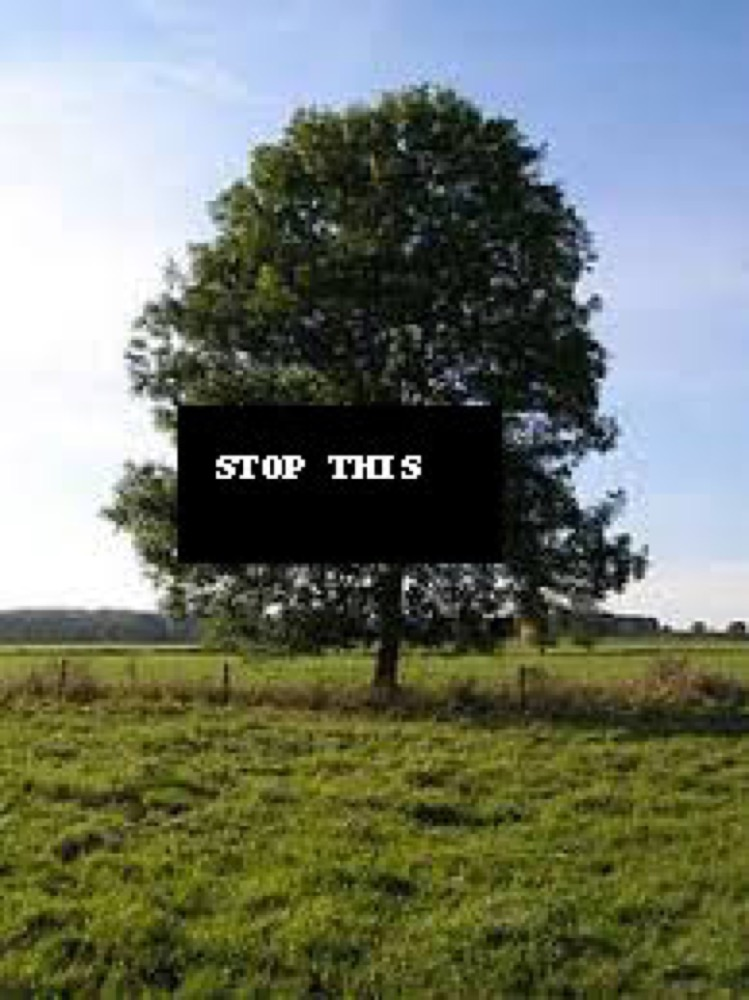
\includegraphics[width=0.75\linewidth,height=0.35\textheight,keepaspectratio]{images/protestpy.jpg}
  \caption{protestpy image for protesting against trees}
  \caption*{Screen capture by myself}
  \label{fig:protestpy-tree}
\end{figure}

Publishing my libraries so they can be installed with one-click, or a command line, and making them depend on other libraries and languages, is for me an exercise in trust, and a way to give back to other artists what I have learned. It is to me like building a skatepark or a hiking trail, you build infrastructure so that other people can use it for their own needs, mostly for fun and art :)

Apart from these software libraries, I have on and off made small publishing experiments other ecosystems, such as Max, Haskell, and Node.js, but the bulk of my work since 2016 is published as Git repositories on my GitHub at \url{https://github.com/montoyamoraga/}.

\begin{figure}[ht]
  \centering
  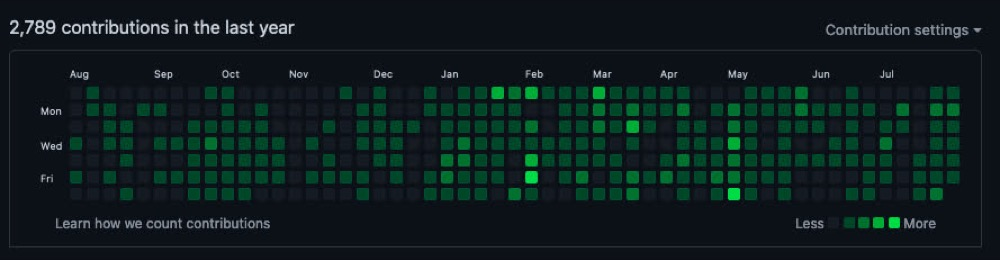
\includegraphics[width=0.80\linewidth,height=0.40\textheight,keepaspectratio]{images/github-contributions.jpg}
  \caption{Github contributions}
  \caption*{Screen capture by myself}
  \label{fig:github-contributions}
\end{figure}

TinyTrainable is my first library for hardware, and this experience has led me to publish libraries for other projects I have been working on, and also publish alpha releases for libraries that were inspired by this thesis, but that I think are out of scope, so I plan on working on them after graduation.

\section{ML for arts}

My first project in this field was in 2016 with my \acrshort{NYU} \acrshort{ITP} classmate Corbin Ordel, who was a student at Gene Kogan's \acrshort{ML} for Artists class. Together we audited Rebecca Fiebrink's \acrshort{ML} for Musicians and Artists class, available at the Kadenze platform, and learned the Wekinator platform. As a final project for Gene's class, with Corbin we made the project Piano Die Hard, a digital sculpture consisting on a piano that is watching the trailer for the movie Die Hard, and every time it detects an explosion, it plays music as accompaniment.

\begin{figure}[ht]
  \centering
  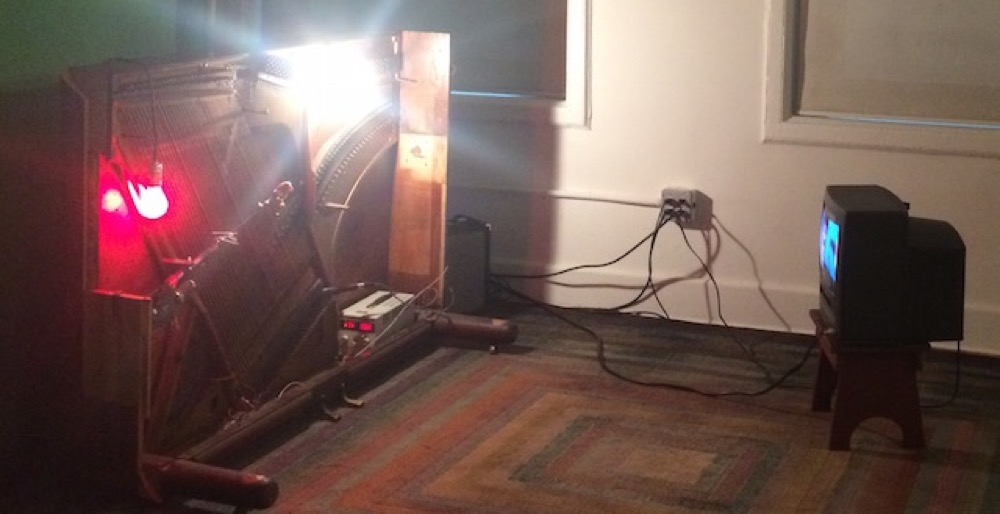
\includegraphics[width=0.80\linewidth,height=0.40\textheight,keepaspectratio]{images/piano-die-hard.jpg}
  \caption{Piano Die Hard}
  \caption*{Retrieved from \cite{website-alt-ai}}
  \label{fig:piano-die-hard}
\end{figure}

The technology stack for this project was very convoluted: a computer looped the trailer of the movie and fed it to an old TV and to an openFrameworks app. This app outputted statistic descriptors about the color of each picture frame, which were then sent to the Wekinator app, which decided with a \acrshort{k-NN} algorithm if the image was either an explosion or not. When it detected an explosion, we sent a control signal to an Arduino, which moved a motor connected to a fishing rod and a kitchen utensil, which scratched the strings of the open carcass of an old piano every time there was explosion.

The training of the model was made beforehand with a selection of 1980's movies, featuring scenes with and without explosions. This project was a direct inspiration for the color input of the TinyTrainable library, mixing color data with a \acrshort{k-NN} algorithm, and it's really fascinating for me to compress all of this complexity of 5 five years ago, needing a computer and different apps, into a single microcontroller, and I hope everybody can enjoy this too.

While graduating from \acrshort{NYU} \acrshort{ITP}, and working for one year as a research resident and graduate teaching assistant, I was exposed to many exciting developments in \acrshort{AI} and creativity, including saw the creation of the the ml5.js library and the company RunwayML by Cristóbal Valenzuela, Alejandro Matamala, and Anastasis Germanidis. Through this I became excited about the creative potential of \acrshort{ML}, so in 2018 I took a month-long intensive class at the School of Machines in Berlin, Germany, facilitated by Gene Kogan and Andreas Refsgaard, and organized by Rachel Uwa.

During this workshop I learned many different tools for \acrshort{ML}, and also did my first experiments in creating my own custom databases. I got a mix from excitement for the graphic and plastic possibilities that \acrshort{AI} gives me, but the main bottleneck that I found was the databases. The algorithms I was trying to play with needed very specific requirements in terms of their data input, such as specific imageresolution, file formats, file size, so even if you found a database, you had to modify it. During this month my work focused on learning how to create databases with web scraping, which you can find at this repository \url{https://github.com.montoyamoraga/scrapers}. This is also the basis for the research in custom databases that I conducted during this research, and my draw towards using the Arduino microcontroller as a source for data, and I hope my contributions in how to parse data and how to build your own databases is helpful to you.

For people that are interested in the rich field of image generation with \acrshort{ML}, I highly recommend the book on GANs by Casey Reas, published by Anteism, as of 2021 on its second edition. It’s an arts-first book that contextualizes the use of \acrshort{ML} algorithms for the creation of images, and uses the metaphor of these algorithms as being similar to the development of the camera. Artists don’t need to understand all the physics or mechanics behind a camera in order to make art with it, but it can help to understand it too. I think that \acrshort{ML} is a revolutionary strategy for instrument making and arts, while also introducing new civic complexities, and in this thesis I have tried to follow the example of this book, to introduce the technology and contextualize for a new generation of artists and instrument makers.
